% Generated by paper/generate_figures.py. Do not edit by hand.
% Source: benchmarks/results/20261127T033045Z/measurements.jsonl
\begin{figure*}[t]
  \centering
  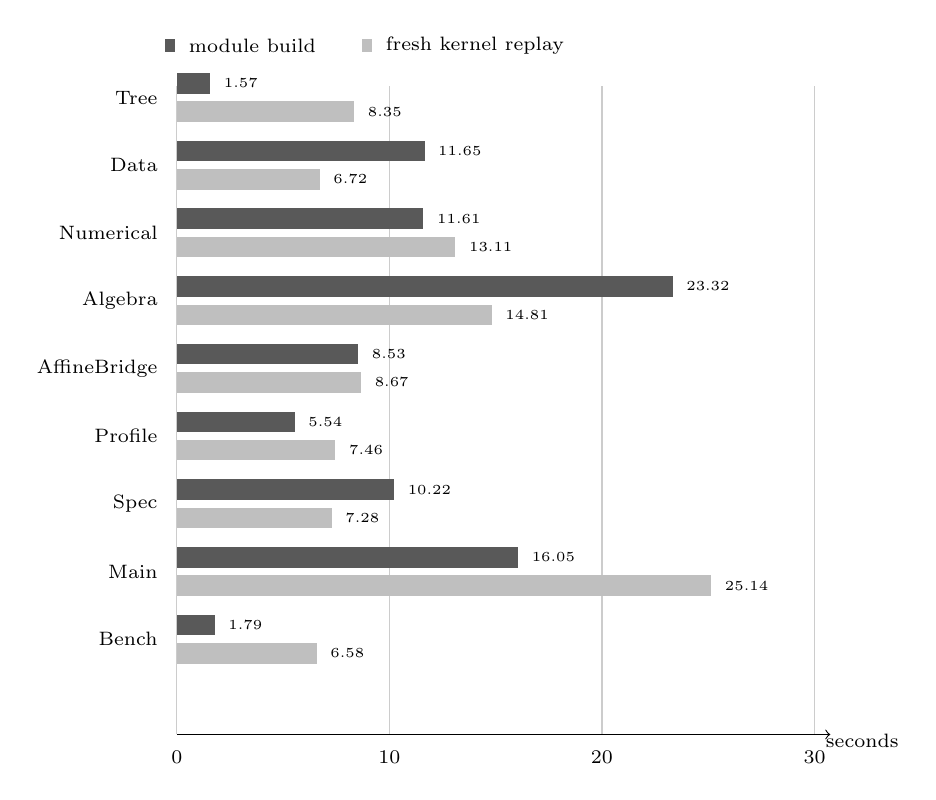
\begin{tikzpicture}[x=1cm,y=1cm,font=\scriptsize]
    \draw[black!20] (0.000,-0.350) -- (0.000,7.890);
    \node[anchor=north] at (0.000,-0.430) {0};
    \draw[black!20] (2.700,-0.350) -- (2.700,7.890);
    \node[anchor=north] at (2.700,-0.430) {10};
    \draw[black!20] (5.400,-0.350) -- (5.400,7.890);
    \node[anchor=north] at (5.400,-0.430) {20};
    \draw[black!20] (8.100,-0.350) -- (8.100,7.890);
    \node[anchor=north] at (8.100,-0.430) {30};
    \draw[->] (0,-0.350) -- (8.300,-0.350);
    \node[anchor=west] at (8.120,-0.430) {seconds};
    \fill[black!65] (-0.15,8.320) rectangle (-0.02,8.480);
    \node[anchor=west] at (0.03,8.400) {module build};
    \fill[black!25] (2.35,8.320) rectangle (2.48,8.480);
    \node[anchor=west] at (2.53,8.400) {fresh kernel replay};
    \node[anchor=east] at (-0.12,7.740) {Tree};
    \fill[black!65] (0,7.790) rectangle (0.425,8.050);
    \node[font=\tiny,anchor=west] at (0.475,7.920) {1.57};
    \fill[black!25] (0,7.430) rectangle (2.253,7.690);
    \node[font=\tiny,anchor=west] at (2.303,7.560) {8.35};
    \node[anchor=east] at (-0.12,6.880) {Data};
    \fill[black!65] (0,6.930) rectangle (3.146,7.190);
    \node[font=\tiny,anchor=west] at (3.196,7.060) {11.65};
    \fill[black!25] (0,6.570) rectangle (1.814,6.830);
    \node[font=\tiny,anchor=west] at (1.864,6.700) {6.72};
    \node[anchor=east] at (-0.12,6.020) {Numerical};
    \fill[black!65] (0,6.070) rectangle (3.133,6.330);
    \node[font=\tiny,anchor=west] at (3.183,6.200) {11.61};
    \fill[black!25] (0,5.710) rectangle (3.538,5.970);
    \node[font=\tiny,anchor=west] at (3.588,5.840) {13.11};
    \node[anchor=east] at (-0.12,5.160) {Algebra};
    \fill[black!65] (0,5.210) rectangle (6.297,5.470);
    \node[font=\tiny,anchor=west] at (6.347,5.340) {23.32};
    \fill[black!25] (0,4.850) rectangle (4.000,5.110);
    \node[font=\tiny,anchor=west] at (4.050,4.980) {14.81};
    \node[anchor=east] at (-0.12,4.300) {AffineBridge};
    \fill[black!65] (0,4.350) rectangle (2.304,4.610);
    \node[font=\tiny,anchor=west] at (2.354,4.480) {8.53};
    \fill[black!25] (0,3.990) rectangle (2.340,4.250);
    \node[font=\tiny,anchor=west] at (2.390,4.120) {8.67};
    \node[anchor=east] at (-0.12,3.440) {Profile};
    \fill[black!65] (0,3.490) rectangle (1.497,3.750);
    \node[font=\tiny,anchor=west] at (1.547,3.620) {5.54};
    \fill[black!25] (0,3.130) rectangle (2.014,3.390);
    \node[font=\tiny,anchor=west] at (2.064,3.260) {7.46};
    \node[anchor=east] at (-0.12,2.580) {Spec};
    \fill[black!65] (0,2.630) rectangle (2.759,2.890);
    \node[font=\tiny,anchor=west] at (2.809,2.760) {10.22};
    \fill[black!25] (0,2.270) rectangle (1.967,2.530);
    \node[font=\tiny,anchor=west] at (2.017,2.400) {7.28};
    \node[anchor=east] at (-0.12,1.720) {Main};
    \fill[black!65] (0,1.770) rectangle (4.334,2.030);
    \node[font=\tiny,anchor=west] at (4.384,1.900) {16.05};
    \fill[black!25] (0,1.410) rectangle (6.788,1.670);
    \node[font=\tiny,anchor=west] at (6.838,1.540) {25.14};
    \node[anchor=east] at (-0.12,0.860) {Bench};
    \fill[black!65] (0,0.910) rectangle (0.482,1.170);
    \node[font=\tiny,anchor=west] at (0.532,1.040) {1.79};
    \fill[black!25] (0,0.550) rectangle (1.776,0.810);
    \node[font=\tiny,anchor=west] at (1.826,0.680) {6.58};
  \end{tikzpicture}
  \caption{Wall times for distinct ordinary construction and
  fresh-process kernel-replay commands. Each bar is one observed
  command. The table aggregates those same commands by phase.}
  \label{fig:timing}
  \Description{A horizontal grouped bar chart. Eight rows correspond
  to the core proof modules and a ninth to the benchmark module;
  each row shows one module-build time and one fresh-process kernel
  replay time in seconds.}
\end{figure*}
